\chapter{FDTD Methods and Analysis Techniques}\label{ch:FDTD}

\begin{flushright}{\it
``Since Newton, mankind has come to realize that the laws of physics\\
are always expressed in the language of differential equations.''\\
- Steven Strogatz} %\\
%\SWcomment[(https://youtu.be/O85OWBJ2ayo?t=44)]
\end{flushright}
%
\vspace{2em}
This chapter introduces some important concepts needed to understand the physical models presented later on in this document. 
By means of a simple mass-spring system and the 1D wave equation, the notation and terminology used throughout this document will be explained, together with some important analysis techniques. 
Before diving into the mathematics, let us go over some useful terminology.

\section{Differential Equations}
Differential equations are used to describe the motion of dynamic systems including vibrations in musical instruments. In this work, these equations are used, among others, to describe the movement of a string, an instrument body and the air pressure in an acoustic tube.

A characteristic feature of these equations is that, rather than an absolute value or \textit{state} of a system, the time derivative of its state -- its velocity -- or the second time derivative -- its acceleration -- is described. From this, the absolute state of the system can then be computed.
%
This state is usually described by the variable $u$ which is (nearly) always a function of time, i.e., $u=u(t)$. If the system is distributed in space, $u$ also becomes a function of space, i.e., $u = u(x,t)$, or with two spatial dimensions, $u = u(x,y,t)$, etc. Though this work only describes systems of up to two spatial dimensions, one can easily extend to three dimensions \cite{Hamilton2016} and potentially higher-dimensional systems \cite{Bustamante2017}\todo{maybe not such a relevant reference..}! 
% one could potentially extend to systems of infinite spatial dimensions evolving over time!

If $u$ is univariate, and only a function of time, the differential equation that describes the motion of this system is called an \textit{ordinary differential equation} (ODE). Various ways to describe the second derivative in time of $u$, or the acceleration of $u$ are
%
\begin{equation}\nonumber
    \begin{aligned}
        \frac{d^2 u}{d t^2} & \quad \text{(Leibniz's notation)},\\
        \ddot u\ \  &\quad \text{(Newton's notation)},\\[3pt]
        D_t^2 u& \quad \text{(Euler's notation)}.
    \end{aligned}
\end{equation}
%
Leibniz' notation could be considered the most standard notation but is not necessarily compact. Newton's notation on the other hand allows for an ultra compact notation using a dot above the function to denote a derivative. However, this notation can only be used for univariate functions which it will be used for in this document. Finally, Euler's notation uses an operator which can be applied to a function and indicates a derivative.  
 
If $u$ is also a function of at least one spatial dimension, the equation of motion is a called a \textit{partial differential equation} (PDE).
The literature uses different types of notation for taking (continuous-time) partial derivatives. Applied to a state variable $u$ these can look like 
\begin{equation}\nonumber
    \begin{aligned}
        \frac{\partial^2 u}{\partial t^2} & \quad \text{(Leibniz's notation)}\\
        u_{tt}\:\,& \quad \text{(subscript notation)}\\[3pt]
        \ptt u\: & \quad \text{(Euler's notation)}
    \end{aligned}
\end{equation}
% 
%
% \begin{equation}\nonumber
%     \begin{aligned}
%         \frac{\partial^2 u}{\partial t^2}, \quad
%         u_{tt},\quad
%         \ptt u
%     \end{aligned}
% \end{equation}
%
where the subscript notation could be seen as the partial derivative counterpart to Newton's notation due to its compactness. In the remainder of this document, the operator notation will be used, due to their similarity to the discrete operators (introduced shortly) and as it allows for creation of bigger operators for more compactness when working with multiple (connected) systems (see e.g. Chapter \ref{ch:tromba}).
Often-used partial derivatives and their meanings \todo{maybe not yet as this is super general still} are shown below

\begin{minipage}[c]{0.49\textwidth}
    \begin{align*}
        \ptt u &\quad \text{(acceleration)}\\
        \pt u &\quad \text{(velocity)}
    \end{align*}
\end{minipage}
\begin{minipage}[c]{0.49\textwidth}
    \begin{align*}
    \pxx u &\quad \text{(curvature)}\\
    \px u &\quad \text{(slope)}
    \end{align*}
\end{minipage}
\subsubsection{Note on dimensions \todo{not done}}
It is important to notice that there is a difference between a system described over multiple spatial dimensions, such as a membrane, or a plate, and a system state having multiple coordinates. In much of the literature on FDTD methods in the field of musical acoustics, the state variable only describes one coordinate. In most string models, for example, only the transverse displacement is considered (see Chapter \ref{ch:stiffString}) and the longitudinal motion of the string is ignored. In other words, every point along the string can only move up and down, not side-to-side. Although this greatly simplifies the system at hand, this is not what happens in reality, and effects such as phantom partials and pitch glides due to tension modulation are not present in the simplified model. 

Models exist that take longitudinal vibration into account... SOTA

Luckily, these single-polarisation models (under low amplitudes) already give 

though work has been done on strings with dual polarisation \cite{Desvages2016}
In this work,  
\textit{Note: difference between 1D, 2D spatial, and 1D, 2D displacement (polarisation). Transverse displacement of 1D wave here}

\section{Discretisation using FDTD methods}
Differential equations are powerful tools that describe the motion of physical systems. Despite this, only few of these have a closed-form \SWcomment[or analytical] solution (such as the simpler ones that will be presented in this chapter). More complex systems require methods that do not perfectly solve, but rather \textit{approximate} the solutions to these equations. Finite-difference time-domain (FDTD) are considered one of the
in terms of generality and flexibility... 

\SWcomment[It is important to note that a discrete FD scheme is an \textit{approximation} to a continuous PDE, not a sampled version of it. This means that the resulting schemes are rarely an exact solution to the original continuous equation.]

These methods essentially subdivide a continuous differential equation into discrete points in time and space, a process called \textit{discretisation}. Once an ODE or PDE is discretised using these methods it is now called a \textit{finite-difference (FD) scheme} which approximates the original differential equation. 

\begin{figure}[h]
    \centering
    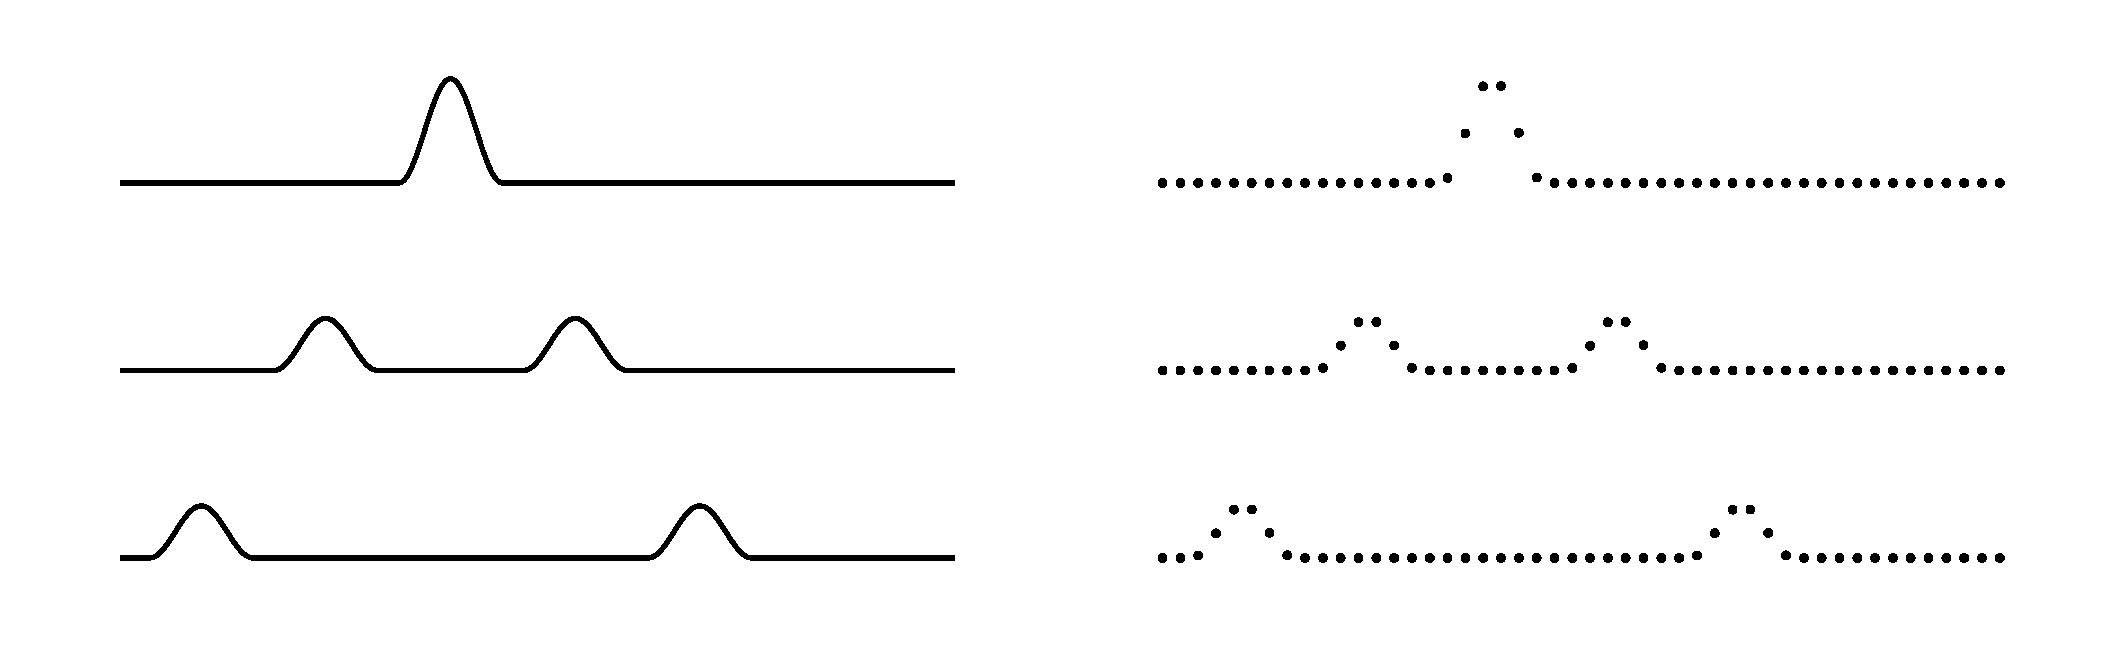
\includegraphics[width=\textwidth]{figures/fdtd/gridFigure.eps}
    \caption{\label{fig:discretisation} \SWcomment[figure visualising discretising a PDE to FDS] }
\end{figure}

\subsection{Grid Functions \todo{check capitalisation of headings throughout document}}
We start by defining a discrete \textit{grid} over time and space which we will use to approximate our continuous equations \todo{grid figure}. A system $u = u(x,t)$ defined over time $t$ and one spatial dimension $x$, can be approximated using a \textit{grid function} $u_l^n$. Here, subscript $l$ and superscript $n$ describe the spatial and temporal indices respectively and arise from the discretisation of the continuous variables $x$ and $t$ according to $x=lh$ and $t=nk$. The spatial step $h$, also called the \textit{grid spacing} describes the distance (in m) between two neighbouring grid points and the temporal step $k$, or \textit{time step} is the time (in s) between two consecutive temporal indices. The latter can be calculated $k=1/\fs$ for a sample rate $\fs$ (in Hz). In many audio applications $\fs = 44100$ Hz which will be used in this work (unless denoted otherwise).

\todo{this might be unnecessary, but I thought that it might be nice to have this in an equation for clarity} To summarise
\begin{equation}
    u(x,t) \approx u_l^n \quad \text{with} \quad x=lh \quad \text{and} \quad t = nk
\end{equation}

\subsection{Finite-Difference Operators}\label{sec:FDoperators}
Now that the state variable has a discrete counterpart, this leaves the derivatives to be discretised, or approximated. We start by introducing shift operators that can be applied to a grid function and `shifts' its indexing, either spatial or temporal. Forward and backward shifts in time, together with the identity operation are
% 
\begin{equation}
    e_{t+}\uln = u_l^{n+1},\quad e_{t-}\uln = u_l^{n-1}, \quad \text{and} \quad 1\uln = \uln.
\end{equation}
%
Similarly, forward and backward shifts in space are
%
\begin{equation}
    e_{x+}\uln = u_{l+1}^n,\quad \text{and}\quad e_{x-}\uln = u_{l-1}^n.
\end{equation}
%
\todo{many figures for shift and FD operators}These shift operators are rarely used in isolation, though they do appear in energy analysis techniques detailed in Section \ref{sec:energyAnalysis}. The operators do, however, form the basis of commonly used \textit{finite-difference (FD) operators}. The first-order derivative in time can be discretised three different ways. The forward, backward and centred \todo{check centred instead of centered, full document sweep} difference operators are
%
\begin{subnumcases}{\pt \approx\label{eq:discFirstTime}}
        \dtp &$\!\!\!\!\!\!\!\!\!\!\triangleq \frac{1}{k}\left(e_{t+} - 1\right),$\label{eq:forwardTimeOperator}\\
        \dtm &$\!\!\!\!\!\!\!\!\!\!\triangleq \frac{1}{k}\left(1 - e_{t-}\right),$\label{eq:backwardTimeOperator}\\
        \dtd &$\!\!\!\!\!\!\!\!\!\!\triangleq \frac{1}{2k}\left(e_{t+} - e_{t-}\right),$\label{eq:centredTimeOperator}
\end{subnumcases}
where ``$\triangleq$'' means ``equal to by definition''. These operators can then be applied to grid function $\uln$ to get
\begin{subnumcases}{\pt u \approx\label{eq:discFirstTimeU}}
    \dtp \uln &$\!\!\!\!\!\!\!\!\!\! = \frac{1}{k}\left(u_l^{n+1} - \uln\right),$\label{eq:forwardTimeOperatorU}\\
    \dtm \uln &$\!\!\!\!\!\!\!\!\!\! = \frac{1}{k}\left(\uln - u_l^{n-1}\right),$\label{eq:backwardTimeOperatorU}\\
    \dtd \uln &$\!\!\!\!\!\!\!\!\!\! = \frac{1}{2k}\left(u_l^{n+1} - u_l^{n-1}\right),$\label{eq:centredTimeOperatorU}
\end{subnumcases}
and all approximate the first-order time derivative of $u$. Note that the centred difference has a division by $2k$ as the time difference between $n+1$ and $n-1$ is, indeed, twice the time step. 

\todo{figure here visualising operators (with reference to grid figure)}
Similar operators exist for a first-order derivative in space, where the forward, backward and centred difference are
\begin{subnumcases}{\px \approx\label{eq:discFirstSpace}}
    \dxp &$\!\!\!\!\!\!\!\!\!\!\triangleq \frac{1}{h}\left(e_{x+} - 1\right),$\label{eq:forwardSpaceOperator}\\
    \dxm &$\!\!\!\!\!\!\!\!\!\!\triangleq \frac{1}{h}\left(1 - e_{x-}\right),$\label{eq:backwardSpaceOperator}\\
    \dxd &$\!\!\!\!\!\!\!\!\!\!\triangleq \frac{1}{2h}\left(e_{x+} - e_{x-}\right),$\label{eq:centredSpaceOperator}
\end{subnumcases}
and when applied to $\uln$ are
\begin{subnumcases}{\px u \approx\label{eq:discFirstSpace}}
    \dxp \uln&$\!\!\!\!\!\!\!\!\!\!= \frac{1}{h}\left(u_{l+1}^n- \uln\right),$\\
    \dxm \uln&$\!\!\!\!\!\!\!\!\!\!= \frac{1}{h}\left(\uln - u_{l-1}^n\right),$\\
    \dxd \uln&$\!\!\!\!\!\!\!\!\!\!= \frac{1}{2h}\left(u_{l+1}^n - u_{l-1}^n\right).$\label{eq:centredSpaceOperatorU}
\end{subnumcases}
Higher order differences can be approxmated through a composition of first-order difference operators. The second-order difference in time may be approximated using
\begin{equation}\label{eq:discSecondTime}
    \ptt \approx \dtp\dtm = \dtt \triangleq \frac{1}{k^2}\left(e_{t+}-2+e_{t-}\right),
\end{equation}
where ``$2$'' is the identity operator applied twice.  and similarly for the second-order difference in space
\begin{equation}\label{eq:discSecondSpace}
    \pxx \approx \dxp\dxm = \dxx \triangleq \frac{1}{h^2}\left(e_{x+}-2+e_{x-}\right).
\end{equation}
Further information on combining operators can be found in Section \ref{sec:combiningOperators}.

Also useful \todo{in energy analysis, interleaved grids, etc.} are averaging operators, all of which approximate the identity operator. The temporal forward, backward and centred averaging operators are
\begin{subnumcases}{1 \approx \label{eq:averagingTime}}
    \mtp & $\!\!\!\!\!\!\!\!\!\!\triangleq \frac{1}{2}\left(e_{t+} + 1\right),$\label{eq:forwardAvgTime}\\
    \mtm & $\!\!\!\!\!\!\!\!\!\!\triangleq \frac{1}{2}\left(1 + e_{t-}\right),$\label{eq:backwardAvgTime}\\
    \mtd & $\!\!\!\!\!\!\!\!\!\!\triangleq \frac{1}{2}\left(e_{t+} + e_{t-}\right).$\label{eq:centredAvgTime}
\end{subnumcases}
Notice how these definitions are different than the difference operators in \eqref{eq:discFirstTime}: the terms in the parentheses are added rather than subtracted, and rather than a division by the time step $k$ there is a division by $2$. Finally, the centred averaging operator does not have an extra division by $2$ as in \eqref{eq:centredTimeOperator}.
Applied to $\uln$, Eqs. \eqref{eq:averagingTime} become
\begin{subnumcases}{\uln \approx \label{eq:averagingTimeU}}
    \mtp \uln & $\!\!\!\!\!\!\!\!\!\!= \frac{1}{2}\left(u_l^{n+1}+ \uln\right),$\label{eq:forwardAvggTimeU}\\
    \mtm \uln & $\!\!\!\!\!\!\!\!\!\!= \frac{1}{2}\left(\uln + u_l^{n-1}\right),$\label{eq:backwardAvggTimeU}\\
    \mtd \uln & $\!\!\!\!\!\!\!\!\!\!= \frac{1}{2}\left(u_l^{n+1} + u_l^{n-1}\right).$\label{eq:centredAvggTimeU}
\end{subnumcases}
%
Similarly, spatial averaging operators are
\begin{subnumcases}{1 \approx \label{eq:averagingSpace}}
    \mxp & $\!\!\!\!\!\!\!\!\!\!\triangleq \frac{1}{2}\left(e_{x+} + 1\right),$\label{eq:forwardAvgSpace}\\
    \mxm & $\!\!\!\!\!\!\!\!\!\!\triangleq \frac{1}{2}\left(1 + e_{x-}\right),$\label{eq:backwardAvgSpace}\\
    \mxd & $\!\!\!\!\!\!\!\!\!\!\triangleq \frac{1}{2}\left(e_{x+} + e_{x-}\right),$\label{eq:centredAvgSpace}
\end{subnumcases}
and when applied to $\uln$
\begin{subnumcases}{\uln \approx \label{eq:averagingSpaceU}}
    \mxp \uln & $\!\!\!\!\!\!\!\!\!\!= \frac{1}{2}\left(u_{l+1}^n+ \uln\right),$\label{eq:forwardAvgSpaceU}\\
    \mxm \uln & $\!\!\!\!\!\!\!\!\!\!= \frac{1}{2}\left(\uln + u_{l-1}^n\right),$\label{eq:backwardAvgSpaceU}\\
    \mxd \uln & $\!\!\!\!\!\!\!\!\!\!= \frac{1}{2}\left(u_{l+1}^n + u_{l-1}^n\right).$\label{eq:centredAvgSpaceU}
\end{subnumcases}
Operators and derivatives in 2D will be discussed in Chapter \ref{ch:2Dsyst}.


\subsubsection{Accuracy}
As FDTD methods approximate continuous systems, the resulting solution is rarely 100\% accurate. To determine the accuracy of the FD operators above, one can perform a Taylor series analysis. The Taylor series is an infinite sum and its expansion of a function $f$ about a point $a$ is defined as
\begin{equation}
    f(x) = \sum_{n=0}^{\infty} \frac{(x-a)^n}{n!}f^{(n)}(a)
\end{equation}
where superscript $(n)$ denotes the $n$\th derivative of $f$ with respect to $x$. The analysis will be performed on the temporal operators in Eqs. \eqref{eq:discFirstTime} and \eqref{eq:discSecondTime},  but also apply to the spatial operators in Eqs. \eqref{eq:discFirstSpace} and \eqref{eq:discSecondSpace}.

Using continuous function $u=u(t)$ and following Bilbao's ``slight abuse of notation'' in \cite{theBible}, one may apply FD operators to continuous functions according to 
\begin{equation}\label{eq:forwardTimeCont}
    \dtp u(t) = \frac{u(t+k) - u(t)}{k}\ .
\end{equation}
%
Assuming that $u$ is infinitely differentiable, $u(t+k)$, i.e., $u$ at the next time step (but in continuous time), can be approximated using a Taylor series expansion of $u$ about $t$ according to
\begin{equation}\label{eq:taylorStartForward}
    u(t+k) = u(t) + k \dot u + \frac{k^2}{2} \ddot u + \frac{k^3}{6} \dot{\ddot{u}} + \O(k^4).
\end{equation}
Here, (following Newton's notation) the dot describes a single temporal derivative and $\O$ includes additional terms in the expansion. The power of $k$ in the argument of $\O$ describes the order of the error, which is lowest power of $k$ (as $k < 1$). Equation \eqref{eq:taylorStartForward} can be rewritten to 
\begin{align}
    \frac{u(t+k) - u(t)}{k} &= \dot u + \frac{k}{2} \ddot u +\frac{k^2}{6} \dot{\ddot{u}} + \O(k^3),\nonumber\\
    \dot u &= \frac{u(t+k) - u(t)}{k} + \O(k),
\end{align}
is the definition of the forward operator in time in Eq. \eqref{eq:forwardTimeCont} but with an additional error term. Notice that the sign of $\O$ does not matter.
As the power of $k$ in $\O$'s argument determines the order of the error of the approximation, we can conclude that the forward operator is first-order accurate. One can also observe that, as expected, the error gets smaller as the time step $k$ gets smaller and indicates that higher sample rates result in more accurate simulations (through $k=1/\fs$).

We can arrive at a similar result for the backward operator. Applying Eq. \eqref{eq:backwardTimeOperator} to $u$ yields
\begin{equation}
    \dtm u(t) = \frac{u(t) - u(t-k)}{k}
\end{equation}
and performing a Taylor series expansion of $u$ about $t$ yields
\begin{align}
    u(t-k) &= u(t) + (-k) \dot u + \frac{(-k)^2}{2} \ddot u +\frac{(-k)^3}{6}\dot{\ddot{u}} + \O(k^4),\label{eq:taylorStartBackward}\\
    \frac{u(t-k) - u(t)}{k} &= -\dot u + \frac{k}{2} \ddot u - \frac{k^2}{6}\dot{\ddot{u}} + \O(k^3),\nonumber\\
    \dot u &= \frac{u(t) - u(t-k)}{k} + \O(k).
\end{align}

Applying the centred operator in Eq. \eqref{eq:centredTimeOperator} to $u$ yields
\begin{equation}
    \dtd u(t) = \frac{u(t+k) - u(t-k)}{2k},
\end{equation}
indicating that to find the order of accuracy for this operator, both Eqs. \eqref{eq:taylorStartForward} and \eqref{eq:taylorStartBackward} are needed. Subtracting these and filling in their definitions yields
\begin{align}
    u(t+k) - u(t-k) &= 2k\dot u - \frac{2k^3}{6}\dot{\ddot{u}} + 2\O(k^5),\\
    \frac{u(t+k) - u(t-k)}{2k} &= \dot u - \frac{k^2}{6}\dot{\ddot{u}} + \O(k^4),\\
    \dot u &= \frac{u(t+k) - u(t-k)}{2k} + \O(k^2).
\end{align}
Notice that due to several terms cancelling out, the centred difference operator is second-order accurate. 

As a first-order derivative indicates the \textit{slope} of a function, the differences in accuracy between the above operators can be visualised as such (see Figure \ref{fig:taylor}). It can be observed that the derivative approximation of the centred operator much more closely matches the the true derivative of $u$ at $t$.

\begin{figure}[h]
    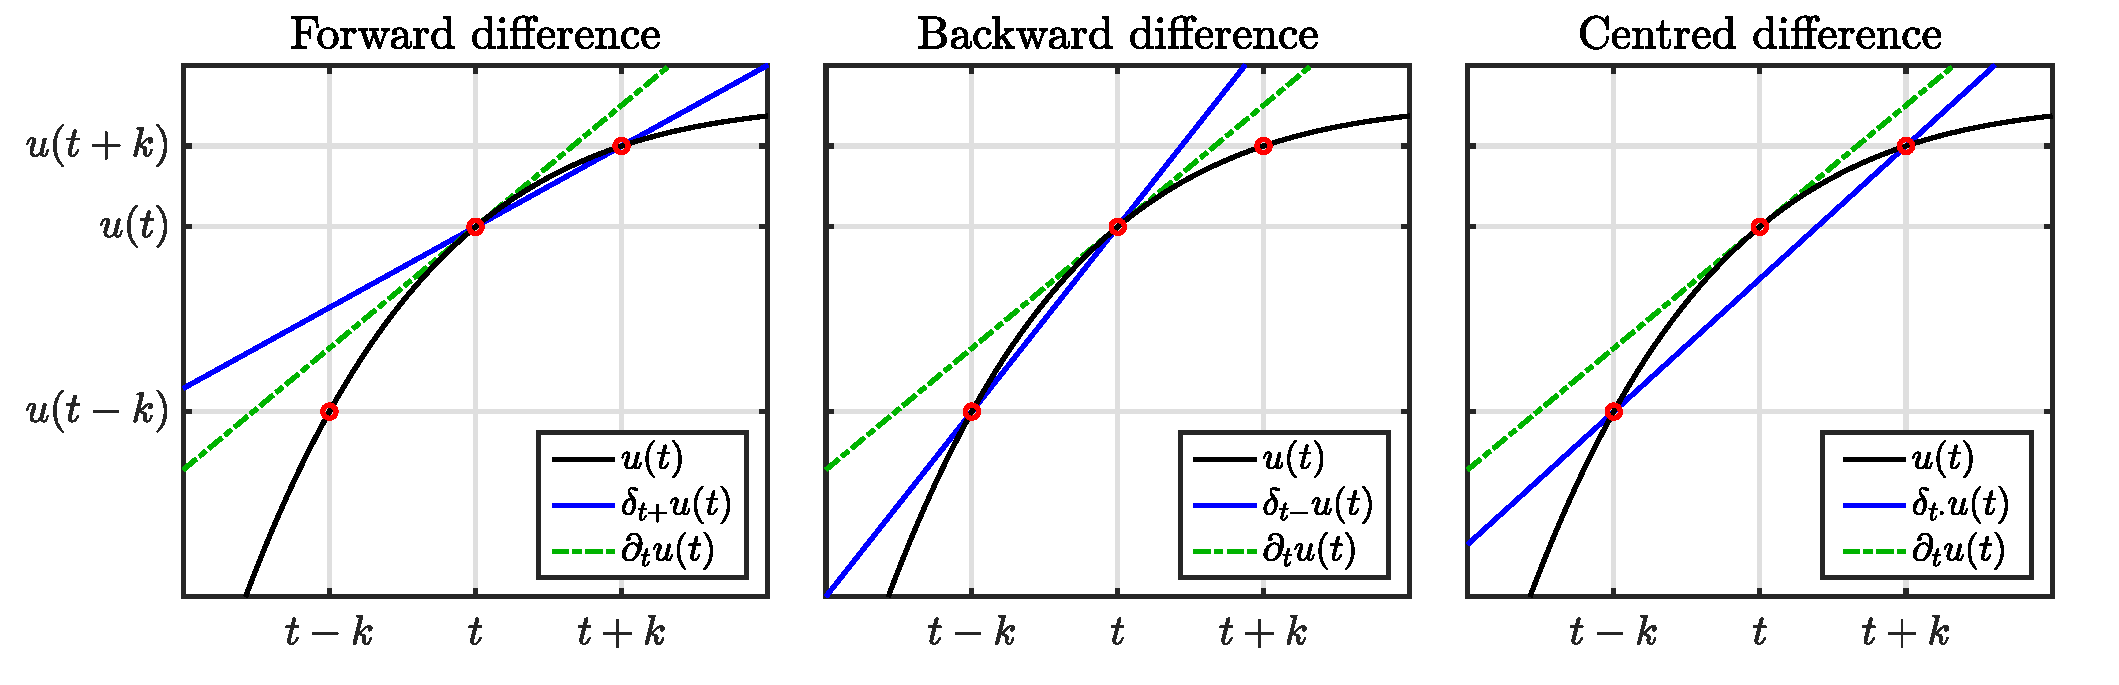
\includegraphics[width=\textwidth]{figures/fdtd/taylor.eps}
    \caption{\label{fig:taylor} The accuracy of the forward, backward and centred difference operators in \eqref{eq:discFirstTime} visualised. One can observe that the centred difference operator much more closely approximates the derivative, or the slope, of $u$ at $t$ than the forward and backward difference operators.}
\end{figure}

Finally, the second-order difference in time operator in Eq. \eqref{eq:discSecondTime} can be proven to be second-order accurate as well by adding Eqs. \eqref{eq:taylorStartForward} and \eqref{eq:taylorStartBackward}:
\begin{align}
    u(t+k) + u(t-k) &= 2 u(t) + k^2 \ddot u + \O(k^4),\nonumber\\
    \frac{u(t+k) -2 u(t) + u(t-k)}{k^2} &= \ddot u + \O(k^2),\nonumber\\
    \ddot u &= \frac{u(t+k) -2 u(t) + u(t-k)}{k^2} + \O(k^2).
\end{align}

\subsection{Identities}
For working with FD schemes, either for implementation or analysis, it can be extremely useful to rewrite the operators presented above to equivalent versions of themselves. These are called idenities and for future reference, some useful ones are listed below
\begin{subequations}
    \begin{align}
        \dtt &= \frac{2}{k}\left(\dtd- \dtm\right)\label{eq:identity1}\\
        \dtd &= \dtp\mtm = \dtm\mtp\label{eq:identity2}\\
        \mtp &= \frac{k}{2}\dtp + 1\label{eq:identity3}
    \end{align}
\end{subequations}
\todo{see whether the negative version of identity \eqref{eq:identity3} is also used later on}
That these equalities hold can easily be proven by expanding the operators defined in Section \ref{sec:FDoperators}. Naturally, these identities also hold for spatial operators by simply substituting the `$t$' subscripts for `$x$'. 

\section{%Intro to ODEs: 
The Mass-Spring System}\label{sec:massSpringSystem}
Though a complete physical modelling field on its own (see Chapter \ref{ch:physMod}), mass-spring systems are also sound-generating systems themselves and lend themselves well to illustrating and explaining FDTD methods in practice. Starting with the continuous-time ODE, this section continues to discretise it to an FD scheme using the operators described in Section \ref{sec:FDoperators}. Finally, the scheme is rewritten to an update equation that can be implemented and the output of the system is shown. 

\subsection{Continuous-time}
Using dots to indicate a temporal derivative, the ODE of a simple mass-spring system is defined as
\begin{equation}\label{eq:massSpringPDE}
    M\ddot u = -Ku,
\end{equation}
where $u = u(t)$ is the distance from the equilibrium position (in m), $M$ \SWcomment[$>0$] is the mass of the mass (in kg) and $K$ \SWcomment[$\geq 0$] is the spring constant (in N/m). In the literature \cite{theBible, }, Eq. \eqref{eq:massSpringPDE} is often written as
\begin{equation}
    \ddot u = -\omega_0^2u
\end{equation}
with 
\begin{equation}\label{eq:omega0MassSpring}
    \omega_0 = \sqrt{K/M}.
\end{equation}
This way of writing the mass-spring ODE is more compact and more straightforward to relate to a fundamental frequency $f_0 = \omega_0 / 2 \pi$ (in Hz). 

Apart from the choices of $K$ and $M$, the behaviour of the mass-spring system is determined by its \textit{initial conditions}, being $u(0)$ and $\pt u(0)$, i.e., the displacement and velocity of the mass at $t = 0$. If the initial conditions are non-zero, the path that the mass follows over time is sinusoidal (see Figure \ref{fig:massSpring}), which is also why the mass-spring system is often referred to as the \textit{simple harmonic oscillator}. The amplitude of the sinusoid is determined by the initial conditions, whereas the frequency is determined by $M$ and $K$. 

\begin{figure}[ht]
    \centering
    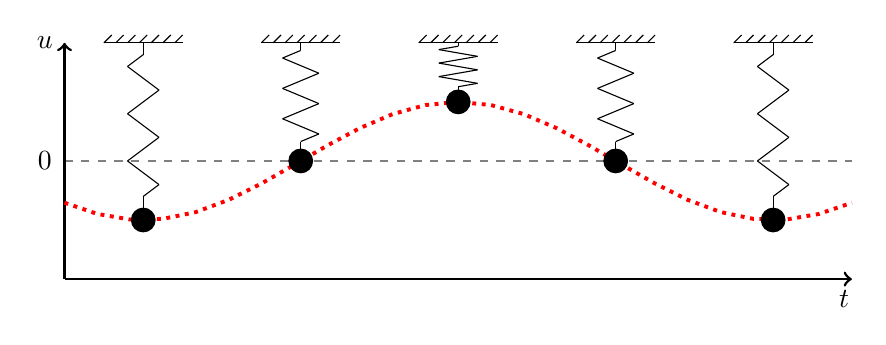
\begin{tikzpicture}
        
        \def\axisLineWidth{0.07};
            
        \def\zigzagLength{0.5}
        \def\zigzags{4}
        \pgfmathsetmacro\halfZigzags{\zigzags/2}
        \def\massSize{0.15}
        \def\massDistanceScaling{2}
        \def\amplitude{0.75}
        
        % axes
        \def\axisOffset{1}
        \draw[dashed, color = gray] (-\axisOffset, 0) -- (4*\massDistanceScaling+\axisOffset, 0);
        \node at (-\axisOffset-0.25, 1.5) {$u$};
        
        %u-axis
        \draw[->, line width=1] (-\axisOffset, -1.5) -- (-\axisOffset, 1.5);

        \node at (-\axisOffset - 0.25, 0) {$0$};

        %t-axis
        \draw[->, line width=1] (-\axisOffset, -1.5) -- (4*\massDistanceScaling+\axisOffset, -1.5);
        
        \node at (4*\massDistanceScaling + \axisOffset-0.1, -1.75) {$t$};

        % sine wave
        \draw[xshift=0 cm, xscale=4, domain=-0.25:2.25, dotted, variable=\x, red, line width=0.05cm] plot ({\x}, {-\amplitude*cos(180*\x)});

        \def\wallHeight{1.5}
        \def\wallHalf{0.5};
        \def\wallLineSpacing{0.15}
        \pgfmathsetmacro\halfNumDiag{\wallHalf / \wallLineSpacing}
        
        \foreach \massNo in {0, ..., 4}
        {
            \def\xshift{\massNo * \massDistanceScaling}

            \begin{scope}[xshift=\xshift cm]
                % draw wall
                \draw[-] (-\wallHalf, \wallHeight) -- (\wallHalf, \wallHeight) node[below, midway] (top) {};
                \foreach \bowDiag in {-\halfNumDiag, ...,\halfNumDiag}
                {
                    \draw[-] (\bowDiag * \wallLineSpacing, \wallHeight) -- (\bowDiag * \wallLineSpacing + 0.1, \wallHeight + 0.1);
                }
                
                \begin{scope}[yshift=1.5cm, rotate=180]
                    %spring extension
                    \pgfmathsetmacro\springHeight{1.5 + \amplitude*cos(\massNo * 90)}
    ;    
                    %what is the step in y
                    \pgfmathsetmacro\yInc{
                        (\springHeight-\massSize)/(2*(\zigzags+1)+4)
                    }

                    %what is the width of the spring based on its extension
                    \pgfmathsetmacro\halfSpringWidth{
                        0.5 * sqrt(\zigzagLength * \zigzagLength - 4 * \yInc * \yInc)
                    }

                    %small dot
                    \filldraw[black] (0, 0) circle (0pt) node[anchor=center](bottomSpring){};    

                    %start of spring
                    \draw[-] (0, 0) -- (0, \yInc);
                    \draw[-] (0, \yInc) -- (\halfSpringWidth, 2*\yInc);

                    % main zig zag
                    \def\curY{2*\yInc};
                    \def\curX{\halfSpringWidth};

                    \foreach \zig in {0, ...,\zigzags}
                    {
                        \pgfmathsetmacro\yToGoTo{\curY+2*\yInc};
                        % \filldraw[black] (0, \yToGoTo) circle (1pt) node[anchor=center](topSpring){\curX};           
                        \draw[-] (\curX, \curY) -- (-\curX, \yToGoTo);
                        \pgfmathsetmacro\tmpX{-\curX};

                        \global\let\curX=\tmpX;
                        \global\let\curY=\yToGoTo;
                    }

                    %end of spring
                    \pgfmathsetmacro\yToGoTo{\curY+\yInc};
                    \draw[-] (\curX, \curY) -- (0, \yToGoTo);
                    \global\let\curY=\yToGoTo;
                    \pgfmathsetmacro\yToGoTo{\curY+\yInc};
                    \draw[-] (0, \curY) -- (0, \yToGoTo);

                    %mass
                    \filldraw[black] (0, \yToGoTo+\massSize) circle (\massSize) node[anchor=center](topSpring){};   
                \end{scope}
            \end{scope}
        }
        % \node at (-0.5, 0.75) (K) {$K$};

    \end{tikzpicture}
    \caption{Mass spring system over time. The system follows a harmonic (sinusoidal) motion. \label{fig:massSpring}}
    \label{fig:lipSystem}
\end{figure}

\subsubsection{Intuition}
The behaviour of the mass-spring system in Eq. \eqref{eq:massSpringPDE} arises from two basic laws of physics: \textit{Newton's second law} and \textit{Hooke's law}. 

Starting with Newton's second law \textit{force equals mass times acceleration}, and relating this to the variables used in Eq. \eqref{eq:massSpringPDE} yields an expression for force
\begin{equation}\label{eq:newton2nd}
    F = M\ddot u.
\end{equation}
This equation in isolation can be used to, fx., calculate the force necessary to accelerate a mass of $M$ kg to $\ddot u$ m/s$^2$. Next, the force generated by the spring follows Hooke's law:
\begin{equation}\label{eq:hookesLaw}
    F = -Ku,
\end{equation} 
which simply states that the force generated by a spring with stiffness $K$ is negatively proportional to the value of $u$. In other words, the further the spring is extended (from the equilibrium $u=0$), the more force will be generated in the opposite direction. Finally, as the sole force acting on the mass is the one generated by the spring, the two expressions for the force $F$ can be set equal to each other and yields the equation for the mass-spring system in \eqref{eq:massSpringPDE}. 

The sinusoidal behaviour of the mass-spring system, or a least the fact that the mass ``gets pulled back'' to the equilibrium, is apparent from the minus-sign in Eq. \eqref{eq:hookesLaw}. The frequency of the sinusoid, depends on the value of $K$ as the ``pull'' happens to a higher degree for a higher spring stiffness. 
That the frequency of the system is also dependent on the mass $M$ can be explained by the fact that a lighter object is more easily moved and vice versa, which is apparent from Eq. \eqref{eq:newton2nd}. In other words, the pull of the spring has a greater effect on the acceleration of a lighter object than a heavier one. 

%Both these parameters affect the frequency through the definition of $\omega_0$ in Eq. \eqref{eq:omega0MassSpring}.

%From the definition of $\omega_0$ in Eq. \eqref{eq:omega0MassSpring} one can observe that a smaller $M$ will cause a higher frequency explained by the fact that a smaller mass is more easily moved. Similarly, a higher spring constant $K$ will cause a higher frequency, as the force caused by Hooke's law ``pulls'' the mass back to the equilibrium to a higher degree.

Finally, if $u = 0$ there is no spring force present and the acceleration remains unchanged. If the mass is not in motion, this means that it remains stationary, but if it is, the velocity is unchanged and it will continue moving with the same speed. 

\subsection{Discrete-time}
The displacement of the mass is approximated using 
\begin{equation}
    u(t) \approx u^n,
\end{equation}
with time $t = nk$, time step $k = 1/\fs$, sample rate $\fs$ and temporal index and $n \in \mathbb{N}^0$.\footnote{In this work, $\mathbb{N}^0$ is used to denote the set of non-negative integers ($\mathbb{N}^0 = 0, 1, 2, 
\hdots$).} Note that the ``grid function'' does not have a subscript $l$ as $u$ is not distributed in space and is now simply called a \textit{time series}.

Using the operators found in Section 
\ref{sec:FDoperators}, Eq. \eqref{eq:massSpringPDE} can be discretised as follows:
\begin{equation}\label{eq:massSpringFDS}
    M \dtt \un = -K\un,
\end{equation}
which is the first appearance of a FD scheme in this work. Expanding the $\delta_{tt}$ operator yields 
\begin{equation*}
    \frac{M}{k^2}\left(u^{n+1}-2\un+u^{n-1}\right) = -K\un,\nonumber
\end{equation*}
and solving for $u^{n+1}$ results in the following recursion or \textit{update equation}:
\begin{equation}\label{eq:massSpringUpdate}
    u^{n+1} = 2\un - u^{n-1} - \frac{Kk^2}{M} u^n,
\end{equation}
which can be implemented in a programming language such as \texttt{MATLAB} or \texttt{C++}. %This is the only unknown value as $u^n$ and $u^{n-1}$ are known from previous calculations. 

To be able to calculate the scheme at $n=0$ (the first time index of the simulation), values must be provided for $u^0$ and $u^{n-1}$. These are determined by the initial conditions. A simple way to obtain a sinusoidal motion with an amplitude of $1$, is to set the initial conditions as follows (using the backwards time difference operator for discretising the first-order time derivative): 
%
\begin{equation}
    u^0 = 1 \quad \text{and} \quad \dtm u^n = 0.
\end{equation}
The latter equality can be solved for $u^{-1}$ to obtain its definition: 
\begin{align*}
    &\frac{1}{k}\left(u^0 - u^{-1}\right) = 0,\\[-1em]
    \xLeftrightarrow{\mystrut\ u^0 = 1\ }\quad &1 - u^{-1} = 0,\\[0.1em]
 &u^{-1} = 1.
\end{align*}
Simply setting $u^0 = u^{-1} \neq 0$ yields an oscillatory behaviour. \todo{maybe a bit short...}

\subsection{Implementation and Output}
A simple \texttt{MATLAB} script implementing the mass-spring system described in this section is shown in Appendix \ref{app:massSpringCode}. The output of the system can be obtained by listening to the displacement of the mass at the given sample rate $\fs$. An example of this can be found in Figure \ref{fig:massSpringOutput} where the frequency of oscillation $f_0 = 440$ Hz.

\begin{figure}[ht]
    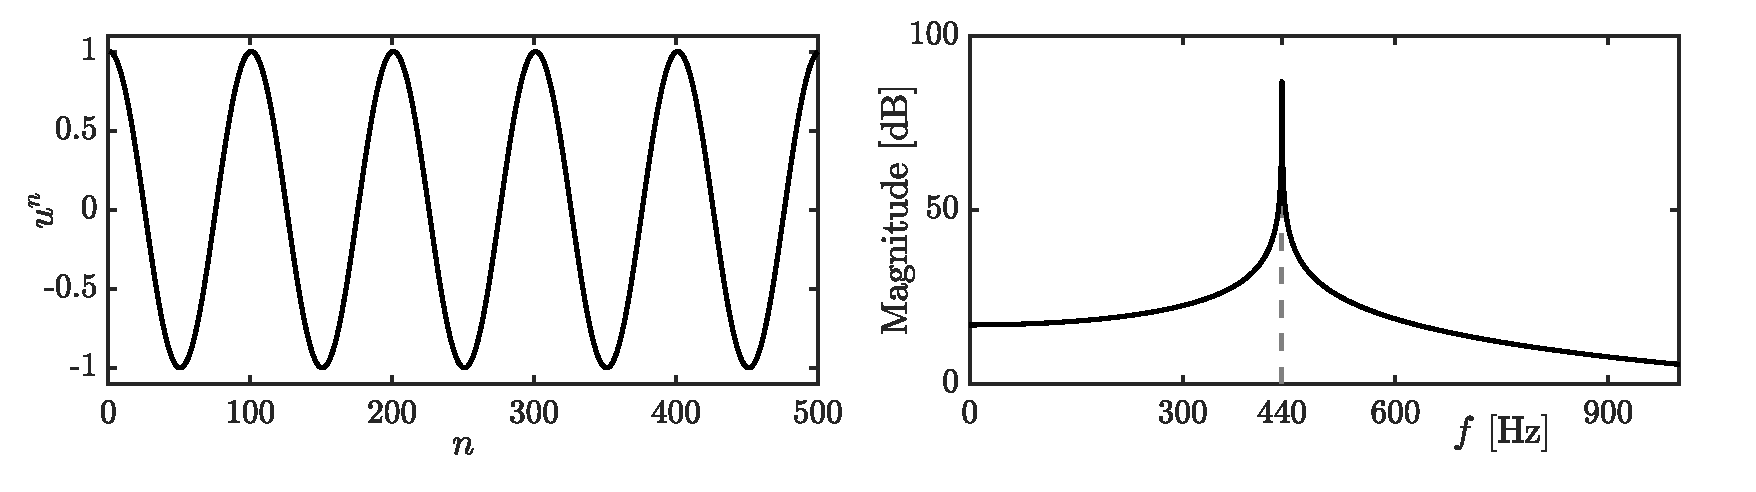
\includegraphics[width=\textwidth]{figures/fdtd/massSpringOutput.eps}
    \caption{The time-domain and frequency-domain output of a mass-spring system with $f_0 = 440$ Hz. \label{fig:massSpringOutput}}
\end{figure}

\todo{Time-domain and FFT figs}

\todo{add damping?}

\section{%Intro to PDEs: 
The 1D Wave Equation}
Arguably the most important PDE in the field of physical modelling for sound synthesis is the 1D wave equation.
\subsection{Continuous-time}
The state of the system $u=u(x,t)$ meaning that is on top of being defined in time $t$ it is distributed over space $x$. The 1D wave equation is defined as follows
\begin{equation}\label{eq:1DwavePDE}
    \ptt u = c^2 \pxx u,
\end{equation}
where $c$ is the wave speed (in m/s). The state variable $u$ can be used to describe transverse vibration in an ideal string, longitudinal vibration in an ideal bar and pressure in an acoustic tube. Although the behaviour of this equation alone does not appear in the real world, as no physical system is ideal, it is extremely useful as a test case and a basis for more complicated models. Here, it will be used to introduce various concepts and analysis techniques in the field of FDTD methods.

\subsubsection{Intuition}
Although the 1D wave equation often appears in the literature, an intuition or interpretation of why it works the way it does is hard to find. In the following, $u$ describes the transverse displacement of an ideal string.

OR 

I would like to use this opportunity to provide some extra explanation as to how and why the 1D wave equation in \eqref{eq:1DwavePDE} works the way it does. This will hopefully provide some basic intuition into the workings of PDEs that will make it easier to work with later on. \SWcomment[somethingsomething]

Going back to Newton's second law

The acceleration of $u = u(x,t)$ at location $x$ is determined by the second-order spatial derivative of $u$ at that same location (scaled by a constant $c^2$). In the case that $u$ describes the transverse displacement of an ideal string, this second-order derivative denotes the \textit{curvature} of this string. As $c^2$ is always positive, the sign (or direction) of the acceleration is fully determined by the sign of the curvature. In other words, a `positive' curvature at location $x$ along the ideal string yields a `positive' or upwards acceleration at that same location. 

What a `positive' or `negative' curvature implies is more easily seen when we take a simple function describing a parabola, $y(x) = x^2$, and take its second derivative to get $y''(x) = 2$. The answer is a positive number which means that $y$ has a positive curvature. 

So, what does this mean for the 1D wave equation? As a positive curvature implies a positive or upwards acceleration as per Eq. \eqref{eq:1DwavePDE}, $u$ with a positive curvature at a location $x$ will start to move upwards and vice versa. Of course, the state of a physical system such as $u$ will rarely have a perfect parabolic shape, but the argument still applies. 

\begin{figure}[h]
    \centering
    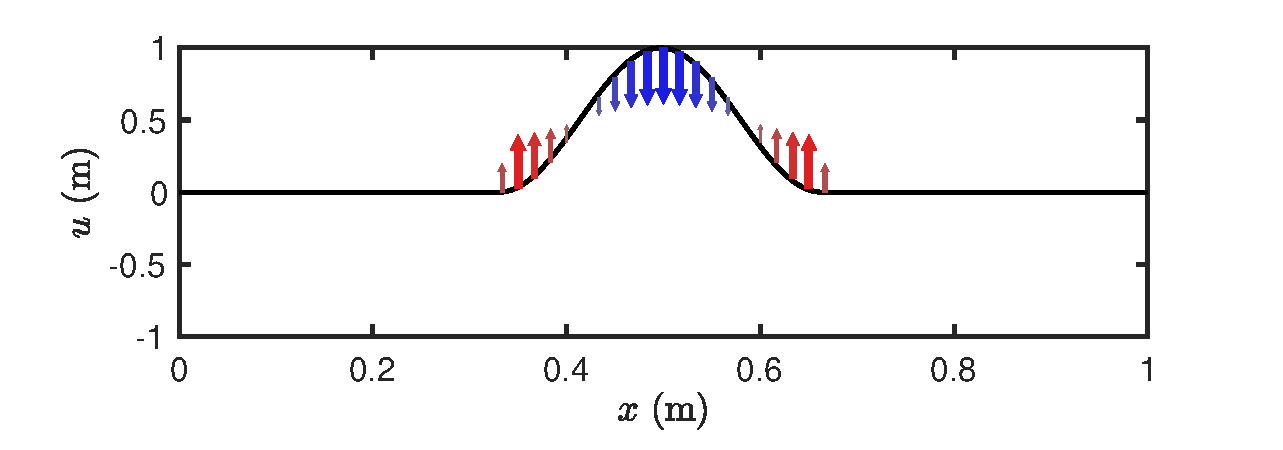
\includegraphics[width=\textwidth]{figures/resonators/curvature.eps}
    \caption{\label{fig:curvature} The forces acting on the 1D wave equation due to curvature. The arrows indicate the direction and magnitude of the force, and simultaneously the acceleration as these are connected through Eq. \eqref{eq:1DwavePDE}.}
\end{figure}\todo{different wording in caption}

\subsubsection{Boundary Conditions}
When a system is distributed in space, 

For analysis purposes, an infinite domain may be adopted, but for implementation, a finite domain needs to be established. 

Consider a system of length $L$ (in m) $x\in \D$ ($x$ is an element in $\D$) where domain $\D = [0, L]$
Two alternatives are

\begin{subequations}\label{eq:boundaryCond1DWave}
    \begin{align}
        u(0, t) = u(L, t) &= 0\quad \text{(Dirichlet, fixed)},\label{eq:contDirichlet}\\
        \px u(0, t) = \px u(L, t) &= 0\quad \text{(Neumann, free)},\label{eq:contNeumann}
    \end{align}
\end{subequations}

\subsection{Discrete-time}
The most straightforward discretisation of Eq. \eqref{eq:1DwavePDE} is the following FD scheme
\begin{equation}\label{eq:1DwaveFDS}
    \dtt \uln = c^2 \dxx \uln.
\end{equation}
Other schemes exist (such as implicit)
\subsubsection{Stability}
The parameters that define \eqref{eq:1DwaveFDS} are linked through a stability condition. The famous Courant-Friedrichs-Lewy or \textit{CFL condition} is defined as \cite{courant} 
\begin{equation}\label{eq:CFL}
    \lambda \leq 1 \quad \text{where} \quad \lambda = \frac{ck}{h}
\end{equation}
where
\begin{equation}\label{eq:courantNumber}
    \lambda = \frac{ck}{h}
\end{equation}
is referred to as the \textit{Courant number}.

Regarding implementation, as the time step $k$ is based on the sample rate and thus usually fixed and $c$ is a user-defined wavespeed, it is useful to rewrite Eq. \eqref{eq:CFL} to be in terms of the grid spacing $h$:
\begin{equation}
    h \geq ck.
\end{equation}
The number of grid points can then be calculated using 
\begin{equation}
    h := ck, \quad N = \floor[\frac{L}{h}], \quad h := \frac{L}{N} \quad \lambda = \frac{ck}{h}.
\end{equation}
where $\floor[\cdot]$ denotes the flooring operation. 

\subsubsection{Implementation}
\begin{equation}\label{eq:1DwaveUpdate}
    u_l^{n+1} = 2 \uln - u_l^{n-1} + \lambda^2 \left(u_{l+1}^n - 2 \uln + u_{l-1}^n\right)
\end{equation}

If $\lambda = 1$, \eqref{eq:1DwaveFDS} is an exact solution to Eq. \eqref{eq:1DwavePDE}. This is no

\subsubsection{Numerical Dispersion}


\subsection{Output}
After the system is excited (see \ref{part:exciters}), one can listen to the output

The location, or frequency of the harmonic partials can also be analytically / numerically derived using modal analysis as will be explained in \ref{sec:modalAnalysis}.
\todo{fft and waveform}

The amplitude of the different modes, on the other hand, depends on the location of excitation and output. 


\subsection{Matrix Form}
For several purposes, such as implementation in MATLAB and several analysis techniques described shortly, is useful to write an FD scheme in \textit{matrix form}. 

In this document, matrices and vectors are written using bold symbols. \SWcomment[Many notations exist, blabla $\bar a$ ] A matrix uses a capital letter whereas vectors are decapitalised. The dimensions of a matrix are denoted using ``$row \times column$''. A $6\times 14$ matrix, for example, thus has $6$ rows and $14$ columns. Along those lines, a \textit{row vector} is a matrix with $1$ row and more than $1$ column and a \textit{column vector} is a matrix with $1$ column and more than $1$ row. \SWcomment[If a matrix has only $1$ row and $1$ column, it can be used as a \textit{scalar}.]

\subsubsection{Matrix Multiplication}
In order for matrix multiplication (including matrix-vector multiplication) to be valid, the number of columns of the first matrix needs to be equal to the number of rows in the second matrix. The result will then be a matrix with a number of rows equal to that of the first matrix and a number of columns equal to that of the second matrix. See Figure \ref{fig:matrixMult} for reference.

As an example, consider the $L
\times M$ matrix $
\A$ and a $M\times N$ matrix $
\B$. The multiplication $\A\B$ is defined as the number of columns of matrix $
\A$ ($M$) is equal to the number of rows of matrix $\B$ (also $M$). The result, $\C$, is a $L \times N$ matrix. The multiplication $\B\A$ is undefined as the number of columns of the first matrix does not match the number of rows in the second matrix. 

Multiplying two matrices written in their dimensions as 
\begin{equation}
    \overbrace{(L\times M)}^{\A}\cdot \overbrace{(M\times N)}^{\B} = \overbrace{(L
    \times N)}^{\C}
\end{equation}
 
\begin{figure}[h]
    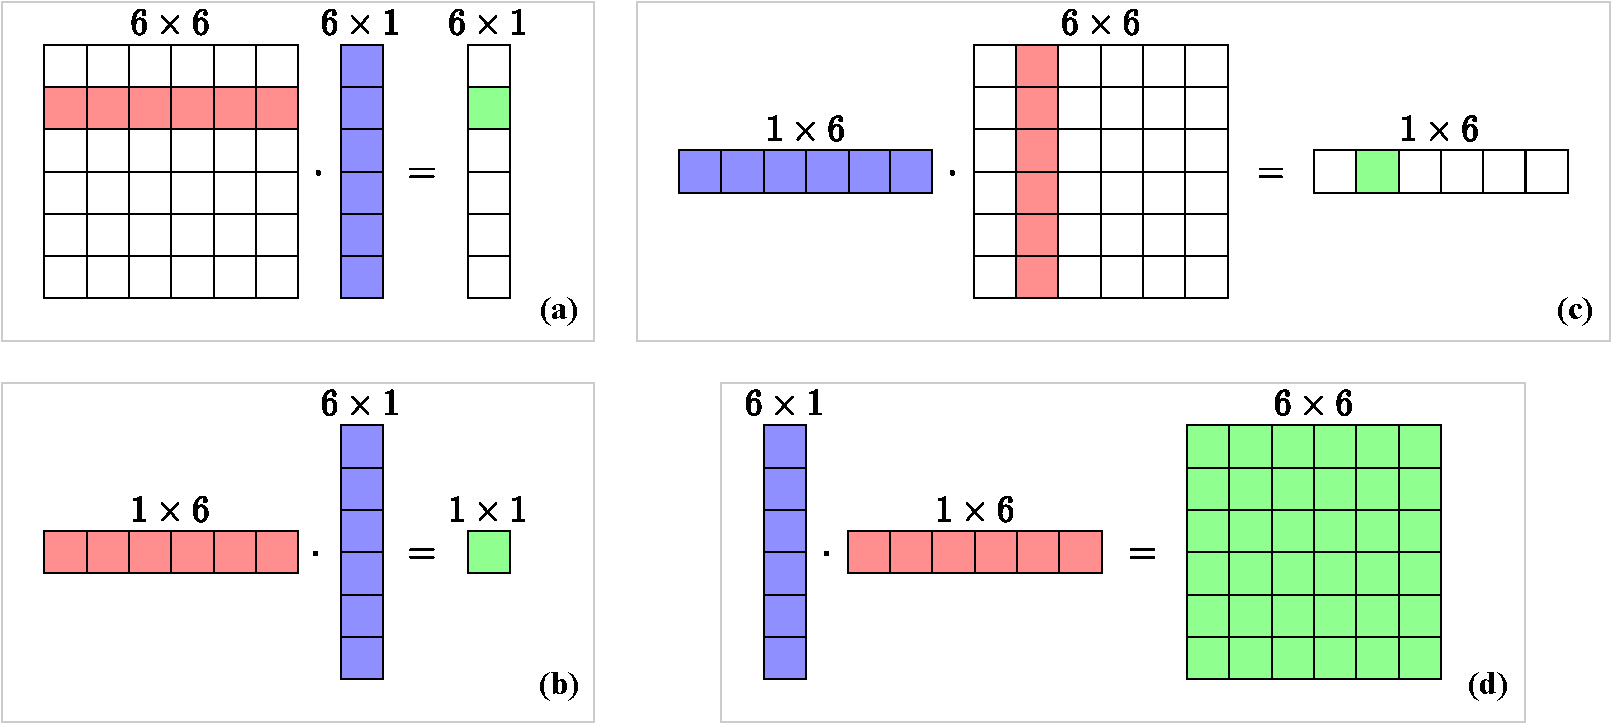
\includegraphics[width=\textwidth]{figures/fdtd/matrixVector2.pdf}
    \caption{Visualisation of valid matrix(-vector) multiplications. \label{fig:matrixVector}}
\end{figure}

\subsubsection{In a FDTD context}
Matrix multiplication when working with FDTD methods usually involves multiplying a square matrix (with equal rows and columns) onto a column vector (see Figure \ref{fig:matrixVector}a). Consider a square matrix with $(N+1)\times (N+1)$ elements $\A$ and a $(N+1) \times 1$ column vector $\u$. Multiplying these results in a $(N+1) \times 1$ column vector $\w$:
\begin{equation}
    \A\u = \w.
\end{equation}
Expanding this operation results in 
\begin{equation}
    \underbrace{\begin{bmatrix}
        a_{00} & a_{01} & \hdots & a_{0N}\\
        a_{10} & a_{11} & \hdots & a_{2N}\\
        \vdots & \vdots & &\vdots\\
        a_{N0} & a_{N1} & \hdots & a_{NN}
    \end{bmatrix}}_{\A}
    \underbrace{\begin{bmatrix}
        u_0\\
        u_1\\
        \vdots\\
        u_N
    \end{bmatrix}}_{\u} = 
    \underbrace{\begin{bmatrix}
        a_{00}u_0 + a_{01}u_1 + \hdots + a_{0N}u_N\\
        a_{10}u_0 + a_{11}u_1 + \hdots + a_{1N}u_N\\
        \vdots\\
        a_{N0}u_0 + a_{N1}u_1 + \hdots + a_{NN}u_N
    \end{bmatrix}}_{\w}
\end{equation}


\subsubsection{Operators in Matrix Form}
The FD operators approximating first-order spatial derivatives in \eqref{eq:discFirstSpace} can be written in matrix form according to
\begin{gather*}\small
    \mathbf{D}_{x+} = \frac{1}{h}\begin{bmatrix}
        \ddots &\ddots & & & \mathbf{0}&\\
         & -1 & 1 & & & \\
        & & -1 & 1 & & \\
        & & & -1 & 1 & \\
        & & & & -1 & \ddots\\
        &\mathbf{0} & & & & \ddots \\
    \end{bmatrix}
    \quad
    \mathbf{D}_{x-} = \frac{1}{h}\begin{bmatrix}
        \ddots & & & & \mathbf{0}&\\
        \ddots & 1 & & & & \\
        & -1 & 1 & & & \\
        & & -1 & 1 & & \\
        & & & -1 & 1 & \\
        &\mathbf{0} & & & \ddots & \ddots \\
    \end{bmatrix}\\
    \\
    \mathbf{D}_{x\cdot} = \frac{1}{2h}\begin{bmatrix}\small
        \ddots &\ddots & & & \mathbf{0}&\\
        \ddots & 0 & 1 & & & \\
        & -1 & 0 & 1 & & \\
        & & -1 & 0 & 1 & \\
        & & & -1 & 0 & \ddots \\
        &\mathbf{0} & & & \ddots & \ddots \\
    \end{bmatrix}\\
\end{gather*}
The matrices $\mathbf{D}_{x+}$ and $\mathbf{D}_{x-}$ can be multiplied to get $\Dxx$:
\begin{equation}\small
    \Dxx = \mathbf{D}_{x+}\mathbf{D}_{x-} = \frac{1}{h^2}\begin{bmatrix}
        \ddots &\ddots & & & \mathbf{0}&\\
        \ddots & -2 & 1 & & & \\
        & 1 & -2 & 1 & & \\
        & & 1 & -2 & 1 & \\
        & & & 1 & -2 & \ddots \\
        &\mathbf{0} & & & \ddots & \ddots \\
    \end{bmatrix}.
\end{equation}
%
Averaging operators $\mxp$, $\mxm$ and $\mxd$ are defined in a similar way:

\begin{gather*}
    \mathbf{M}_{x+} = \frac{1}{2}\begin{bmatrix}
        \ddots &\ddots & & & \mathbf{0}&\\
         & 1 & 1 & & & \\
        & & 1 & 1 & & \\
        & & & 1 & 1 & \\
        & & & & 1 & \ddots\\
        &\mathbf{0} & & & & \ddots \\
    \end{bmatrix}
    \qquad
    \mathbf{M}_{x-} = \frac{1}{2}\begin{bmatrix}
        \ddots & & & & \mathbf{0}&\\
        \ddots & 1 & & & & \\
        & 1 & 1 & & & \\
        & & 1 & 1 & & \\
        & & & 1 & 1 & \\
        &\mathbf{0} & & & \ddots & \ddots \\
    \end{bmatrix}\\
    \\
    \mathbf{M}_{x\cdot} = \frac{1}{2}\begin{bmatrix}
        \ddots &\ddots & & & \mathbf{0}&\\
        \ddots & 0 & 1 & & & \\
        & 1 & 0 & 1 & & \\
        & & 1 & 0 & 1 & \\
        & & & 1 & 0 & \ddots \\
        &\mathbf{0} & & & \ddots & \ddots \\
    \end{bmatrix}\\
\end{gather*}

It is important to notice that only spatial operators are written in this matrix form and then applied to state vectors at different time steps ($n+1$, $n$ and $n-1$). 

Finally, the identity matrix is a matrix with only $1$s on the diagonal and $0$s elsewhere as
\begin{equation}
    \I = \begin{bmatrix}
        \ddots & & & & \mathbf{0}&\\
         & 1 & & & & \\
        & & 1 & & & \\
        & & & 1 & & \\
        & & & & 1 & \\
        &\mathbf{0} & & &  & \ddots \\
    \end{bmatrix}\\
\end{equation}
\subsubsection{Schemes and Update Equations in Matrix Form}
With these building blocks we can write Eq. \eqref{eq:1DwaveFDS} in matrix form. The values of the grid function $\uln$ can be stored in a state vector according to $\u^n = [u_0^n, u_1^n, \hdots, u_N^n]^T$ where $T$ denotes the transpose operation. The FD scheme in \eqref{eq:1DwaveFDS} can then be written in matrix form as
\begin{equation}\label{eq:1DwaveMatrix}
    \frac{1}{k^2}\left(\u^{n+1} - 2 \u + \u^{n-1}\right) = c^2 \Dxx \u^n,
\end{equation}
and rewritten to a matrix form of the update equation
\begin{equation}
    \u^{n+1} = (2\I + c^2k^2 \Dxx )\u^n - \u^{n-1}.
\end{equation}
The identity matrix is necessary here for correct matrix addition.

\subsection{System of Linear Equations}
A number of unknowns described by the same number of equations can be solved using a 


\section{Energy Analysis}\label{sec:energyAnalysis}
Debugging physical models.

\subsection{Mathematical tools}
\subsubsection{Continuous-time}
For two functions $f(x)$ and $g(x)$ and $x\in\D$ their $l_2$ inner product along with the $l_2$ norm is defined as
\begin{equation}\label{eq:contInnerProd}
    \langle f, g\rangle_\D \int_\D fg dx \quad \text{and} \quad \lVert f \rVert_\D = \sqrt{\langle f, f \rangle_\D}
\end{equation}


\subsubsection{Discrete-time}
Inner product of any time series $f^n$ and $g^n$ and the discrete counterpart to \eqref{eq:contInnerProd} is
\begin{equation}\label{eq:discInnerProd}
    \langle f^n, g^n \rangle_\D = \sum_{l\in\D} h f_l^n g_l^n
\end{equation}
where the multiplication by $h$ is the discrete counterpart of $dx$ the continuous definition. 

\subsubsection{Product Identities}
Some useful identities used in this work are
\begin{subequations}
    \begin{align}
        (\dtd \uln)(\dtt \uln) &= \dtp \left(\frac{1}{2}(\dtm \uln)^2\right),\label{eq:prodIdentity1}\\
        (\dtd \uln)\uln &= \dtp \left(\frac{1}{2}\uln e_{t-}\uln\right),\label{eq:prodIdentity2}\\
        (\dtp \uln)(\mtp \uln) &= \dtp \left(\frac{1}{2}(\uln)^2\right),\label{eq:prodIdentity3}\\
        (\dtd \uln)(\mu_{t\cdot}\uln) &= \dtd\left(\frac{1}{2} (\uln)^2\right).\label{eq:prodIdentity4}
    \end{align}
\end{subequations}
Again, these can be used for spatial derivatives as well by substituting the `$t$' subscripts for `$x$'. Also  to 

When an operator is applied to a product of two grid functions, the discrete counter part of the product rule needs to be used according to
\begin{equation}
    \dtp (\uln\wln) = (\dtp \uln)(\mtp\wln) + (\mtp \uln)(\dtp \wln).
\end{equation}
\section{von Neumann Analysis}\label{sec:stabilityAnalysis}
Much literature gives the stability condition using an ``it can be shown that'' argument (fx. \cite{Bilbao2009}). Here, I would like to take the opportunity to 

Finding stability conditions for models

Sin identity:
\begin{equation}\label{eq:sinIdentity}
    \sin(x) = \frac{e^{jx} - e^{-jx}}{2j}\ \ \Rightarrow \ \ \sin^2(x) = \frac{e^{j2x} - 2e^{jx-jx}+ e^{-j2x}}{-4} = \frac{e^{j2x} + e^{-j2x}}{-4} + \frac{1}{2}.
\end{equation}
Cos identity:
\begin{equation}\label{eq:cosIdentity}
    \cos(x) = \frac{e^{jx} + e^{-jx}}{2}\ \ \Rightarrow \ \ \cos^2(x) = \frac{e^{j2x} + 2e^{jx-jx}+ e^{-j2x}}{4} = \frac{e^{j2x} + e^{-j2x}}{4} + \frac{1}{2}.
\end{equation}

One can analyse a \todo{check `a' or `an' FD scheme}FD scheme by 
\begin{equation}
    u_l^n = z^n e^{jl\beta h}
\end{equation}
where $\beta$ is a real wavenumber. Important to remember is that without a shift in space (fx. $l+1$) or time (fx. $n-1$) $l = 0$ or $n=0$ respectively:
\begin{subequations} \label{eq:identitiesZ}
    \begin{align}
        u_l^n &= z^0 e^{j0\beta h} = 1\\
        u_{l+1}^n &= z^0 e^{j1\beta h} = e^{j\beta h}\\
        u_{l-1}^n &= z^0 e^{j(-1)\beta h} = e^{-j\beta h}\\
        u_{l+2}^n &= z^0 e^{j2\beta h} = e^{j\beta h}\\
        u_{l-2}^n &= z^0 e^{j(-2)\beta h}= e^{-j2\beta h}\\
        u_l^{n+1}&= z^1 e^{j0\beta h} = z\\
        u_l^{n-1}&= z^{-1} e^{j0\beta h} = z^{-1}
    \end{align}
\end{subequations}

\todo{Talk about solution of }

\section{Modal Analysis}
\label{sec:modalAnalysis}
Modes are the resonant frequencies of a system. The amout of modes that a discrete system contains dependends on the amount of moving points. A mass-spring system thus has one resonating mode, but a FD scheme of the 1D wave equation with $N = 30$ and Dirichlet boundary conditions will have $29$ modes. This section will show how to obtain the modes of an FD scheme implementing the 1D wave equation. 

We start by using the the matrix form of FD scheme \eqref{eq:1DwaveFDS} from Eq. \eqref{eq:1DwaveMatrix}
\begin{equation*}
    \frac{1}{k^2}\left(\u^{n+1}-2\u^n+\u^{n-1}\right) = c^2 \Dxx\u.
\end{equation*}
Following \cite{theBible} we assume a solution of the form $\u = \boldsymbol{\phi}z^n$ \todo{more explanation}. Substituting this into Eq. \eqref{eq:matrixForm1D} yields the characteristic equation
\begin{equation}
    (z - 2 + z^{-1})\boldsymbol{\phi} = c^2k^2\Dxx \boldsymbol{\phi}.
\end{equation}
This is an eigenvalue problem where the $p$'th solution is defined as 
\begin{gather}
    z_p-2+z_p^{-1} = c^2k^2\text{eig}_p(\Dxx)\nonumber\\
    z_p+(-2-c^2k^2\text{eig}_p(\Dxx))+z_p^{-1}=0
\end{gather}
where $\text{eig}_p(\cdot)$ denoting the $p$th eigenvalue of `$\cdot$'. \SWcomment[If the CFL condition for the scheme is satisfied, the roots will lie on the unit circle.] Furthermore we can substitute a test solution $z_p=e^{j\omega_pk}$ solve for the eigenfrequencies:
\begin{align*}
    e^{j\omega_pk}+e^{-j\omega_pk}-2-c^2k^2\text{eig}_p(\Dxx)&=0\\
    \frac{e^{j\omega_pk}+e^{-j\omega_pk}}{-4}+\frac{1}{2}+\frac{c^2k^2}{4}\text{eig}_p(\Dxx)&=0
\end{align*}
Then using Eq. \eqref{eq:sinIdentity} we get
\begin{align}
    \sin^2(\omega_pk/2)+c^2k^2\text{eig}_p(\Dxx)&=0\nonumber\\
    \sin(\omega_pk/2)&=c k\sqrt{-\text{eig}_p(\Dxx)}\nonumber\\
    \omega_p &= \frac{2}{k}\sin^{-1}\left(c k\sqrt{-\text{eig}_p(\Dxx)}\right)
\end{align}
which is Eq. (6.53) in \cite{theBible}.

\section{Dispersion analysis}\label{sec:dispersionAnalysis}
